\section{The Quantum Integer Comparator}

In this section we are going to analyse a classical circuit that compares two integer numbers
$A$ and $B$ and produces three different signals:

\begin{enumerate}
    \item signal when $A$ is equal with $B$
    \item signal when $A$ is greater than $B$ and
    \item signal when $A$ is less than $B$
\end{enumerate}

\subsection{Analysing the diagram and logic of the classical Comparator circuit}

In the digital logic, a comparator circuit is used to compare two binary encoded numbers. The encoding of (signed or unsigned)
is particularly useful because in the case of the signed-magnitude encoding, we just need to compare the most-significant bits
of the two numbers. If the numbers have different signs then we need only to check their signs, that means their most-significant
bits, and in the later case, when they have the same sign, we need to check their absolute magnitude \cite{Giannakopoulos2015}.

For the purposes of simplicity, we are going to analyze a \textit{serial binary comparator} circuit.

Some classical computers have the capabilities to compute multiple comparison logics like: $>$, $<$, $\ge$, $\le$, $=$ and $\neq$.
Some other computers can only produce a sset of the those comparisons. We are going to analyze only a sset of those comparisons,
specificaly we are going to analyze and construct a digital logic circuit that computes only $=$, $\neq$, $<$ and $>$.
We can produce the truth table of a circuit that computes the equality of two 1-bit numbers easily.

\begin{table}[ht]
    \centering
    \begin{tabular}{cc|c}
        $A$ & $B$ & Equals \\
        \hline
        $0$ & $0$ & $=(1)$ \\
        $0$ & $1$ & $\neq(0)$ \\
        $1$ & $0$ & $\neq(0)$ \\
        $1$ & $1$ & $=(1)$ \\
    \end{tabular}
    \caption{The truth table of a circuit that implements equality check between two bits}
\end{table}

Note that the truth table is equivelant to the XNOR gate's truth table. In fact, if we had $n$-bit inputs, we would just need
$n$ XNOR gates and a $n$-input AND gate to implement a $n$-input equality comparator.

Next, we can implement a circuit that compares two bits and produces $0\text{ when }<$ and $1\text{ when }\geq$

\begin{table}[ht]
    \centering
    \begin{tabular}{cc|c}
        $A$ & $B$ & Greater Equals or Less than \\
        \hline
        $0$ & $0$ & $1(\geq)$ \\
        $0$ & $1$ & $0(<)$ \\
        $1$ & $0$ & $1(\geq)$ \\
        $1$ & $1$ & $1(\geq)$ \\
    \end{tabular}
    \caption{The truth table of a circuit that implements the "greater or equals than" between two bits}
\end{table}

The boolean expression that implements this circuit is the following:

\begin{equation}
    F = A + B'
\end{equation}
Putting it all together we construct the following logic circuit.

\begin{figure}[ht]
    \centering
    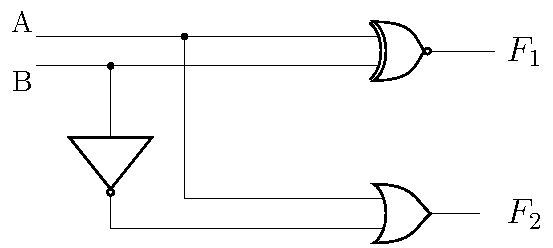
\includegraphics[height=4cm]{images/5_Implementation/classical_1bit_comparator.pdf}
\end{figure}

\begin{equation}
    \text{Where }F_1 =
    \begin{cases}
        A = B, \text{ when }1 \\
        A \neq B, \text { when }0
    \end{cases}
    \text{ and where }
    F_2 =
    \begin{cases}
        A \geq B, \text{ when }1 \\
        A < B, \text{ when }0
    \end{cases}
\end{equation}

\begin{table}[ht]
    \centering
    \begin{tabular}{cc|cc}
        $A$ & $B$ & $F_1$ & $F_2$ \\
        \hline
        $0$ & $0$ & $1$ & $1$ \\
        $0$ & $1$ & $0$ & $0$ \\
        $1$ & $0$ & $0$ & $1$ \\
        $1$ & $1$ & $1$ & $1$ \\
    \end{tabular}
    \caption{The truth table of the classical comparator circuit for two bits}
\end{table}
\newpage
We are going to present the diagram for a quantum comparator of integers. The design is based on the work of Nascimento,
Kowanda and de Oliveira \cite{NKO2006}. The design specifies two important constructs:

\begin{enumerate}
    \item the unitary gate $S$ - a quantum gate that computes the difference of two-qubits
    \item the inverse of the unitary gate $S$, $S^\dag$ - a quantum gate that un-computes the computed difference
\end{enumerate}

We use the $S^\dag$ gate to restore $B$ to its initial state, because $S$ gate computes the difference of $A$ and $B$
and stores it to $B$. Just like the quantum Half-Adder from section 5.1, we un-compute the changes to a particular
qubit so it can be used for some later computation.

\begin{figure}[ht]
    \centering
    \begin{subfigure}{0.3\textwidth}
        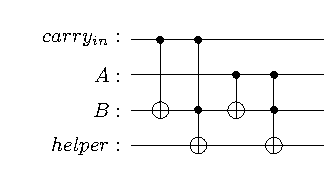
\includegraphics{images/5_Implementation/quantum_nko_sgate.pdf}
        \caption{}
    \end{subfigure}
    \hspace{2.5cm}
    \begin{subfigure}{0.3\textwidth}
        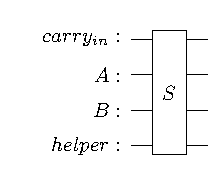
\includegraphics{images/5_Implementation/quantum_nko_sgate_final.pdf}
        \caption{}
    \end{subfigure}
    \begin{subfigure}{0.3\textwidth}
        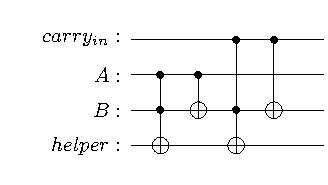
\includegraphics{images/5_Implementation/quantum_nko_sdaggate.pdf}
        \caption{}
    \end{subfigure}
    \hspace{2.5cm}
    \begin{subfigure}{0.3\textwidth}
        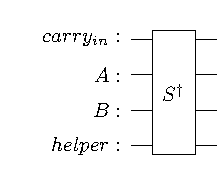
\includegraphics{images/5_Implementation/quantum_nko_sdaggate_final.pdf}
        \caption{}
    \end{subfigure}
    \caption{The unitary $S$ and $S^\dag$ gates' circuit (a, c) and gate (b, d) diagrams}
\end{figure}

To compare two variable-sized quantum registers $A, B$, we need to apply the $S$ gate to 
each pair $A_i,B_i$ and $ancilla_i,ancilla_{i+1}$. Note that we need $n+1$ ancilla qubits
to implement this design. We iteratively apply the above.

Apply a multi-inverse-control CNOT gate to circuit. Control qubits are register $B$'s qubits,
which stores the difference of $A-B$ in 2s-complement, and target the $O_0$ qubit which is the
least-significant qubit of a special purpose register we shall call the \textit{status register}.

Lastly, we copy, by applying a regular CNOT gate, the most-significant qubit of register $B$,
which stores the sign of the difference, to qubit $O_1$ of the status register.

Finally, we uncompute iteratively using the $S^\dag$ gate.

\begin{figure}[ht]
    \centering
    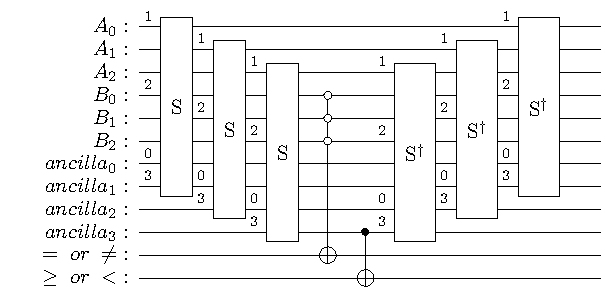
\includegraphics{images/5_Implementation/nko_comparator.pdf}
    \caption{The diagram of the quantum Integer Comparator circuit}
\end{figure}

\subsection{The Python3 Implementation}

To implement the comparator circuit we need to construct the $S$ and $S^\dag$ gates.

\begin{listing}[ht]
    \centering
    \begin{minted}{python3}
        s = QuantumCircuit(4, name="S")
        s.cx(0, 2)
        s.ccx(0, 2, 3)
        s.cx(1, 2)
        s.ccx(1, 2, 3)
        s = s.to_gate()

        sdag = QuantumCircuit(4, name="S_dag")
        sdag.ccx(1, 2, 3)
        sdag.cx(1, 2)
        sdag.ccx(0, 2, 3)
        sdag.cx(0, 2)
        sdag = sdag.to_gate()
    \end{minted}
    \caption{}
\end{listing}

After that we init the main circuit. The size of the registers are fixed to $n=3$, although it can
be set to any positive integer. We also include some ancilla qubits.

\begin{listing}[ht]
    \centering
    \begin{minted}{python3}
        n = 3
        a = QuantumRegister(n, name="A")
        b = QuantumRegister(n, name="B")
        anc = QuantumRegister(n+1, name="ancilla")
        eq = QuantumRegister(1, name="Eq")
        geq = QuantumRegister(1, name="Geq")

        circuit = QuantumCircuit(a, b, anc, eq, gl, name="NKOComparator")
    \end{minted}
    \caption{}
\end{listing}

\newpage

Following the initialization is the main circuit logic. First apply the $S$ gate to compute
the difference of $A-B$ and store it to $B$.

\begin{listing}[ht]
    \centering
    \begin{minted}{python3}
        # compute diff
        for i in range(n):
            circuit.append(s, (anc[i], a[i], b[i], anc[i+1]))
    \end{minted}
    \caption{}
\end{listing}

After we computed the difference, check if all the qubits of register $B$ are zero.
This can be done by using a Multi-Controlled CNOT Gate (MCX) from the \mintinline{python3}|qiskit.circuit.library|.
We set the MCX gate to use inverted logic for the control qubits, so if every control qubit is in the zero state
the target qubit will be inverted. If every qubit of register $B$ are in the zero state, the two registers stored
the same number thus $A$ and $B$ are equal.

\begin{listing}[ht]
    \centering
    \begin{minted}{python3}
        from qiskit.circuit.library import MCXGate
        circuit.append(MCXGate(n, ctrl_state=0), (b[:] + eq[:]))
    \end{minted}
    \caption{}
\end{listing}

To check if $A$ is greater or less than $B$, we can check the sign qubit of the difference. This is easily
done by applying a CNOT gate to most-significant qubit of the difference.

\begin{listing}[!ht]
    \centering
    \begin{minted}{python3}
        circuit.cx(anc[-1], geq)
    \end{minted}
    \caption{}
\end{listing}

\newpage

Finally, we un-compute by applying the $S^\dag$ gate to the circuit in reverse.

\begin{listing}[ht]
    \centering
    \begin{minted}{python3}
        for i in reversed(range(n)):
            circuit.append(sdag, (anc[i], a[i], b[i], anc[i+1]))
    \end{minted}
    \caption{}
\end{listing}

\begin{listing}[ht]
    \centering
    \begin{minted}{python3}
        from qiskit import QuantumCircuit, QuantumRegister

        n = 3

        a = QuantumRegister(n, name="A")
        b = QuantumRegister(n, name="B")
        anc = QuantumRegister(n+1, name="ancilla")
        eq = QuantumRegister(1, name="eq")
        gl = QuantumRegister(1, name="geq")

        circuit = QuantumCircuit(a, b, anc, eq, geq, name="NKOComparator")

        s = QuantumCircuit(4, name="S")
        s.cx(0, 2)
        s.ccx(0, 2, 3)
        s.cx(1, 2)
        s.ccx(1, 2, 3)
        s = s.to_gate()
            
        sdag = QuantumCircuit(4, name="S_dag")
        sdag.ccx(1, 2, 3)
        sdag.cx(1, 2)
        sdag.ccx(0, 2, 3)
        sdag.cx(0, 2)
        sdag = sdag.to_gate()

        # compute diff
        for i in range(n):
            circuit.append(s, (anc[i], a[i], b[i], anc[i+1]))

        from qiskit.circuit.library import MCXGate
        circuit.append(MCXGate(n, ctrl_state=0), (b[:] + eq[:])) # compute equals
        circuit.cx(anc[-1], geq) # if msb < 0 then a < b else b >= a

        # un-compute diff
        for i in reversed(range(n)):
            circuit.append(sdag, (anc[i], a[i], b[i], anc[i+1]))
    \end{minted}
\end{listing}